\chapter[Anexos]{Anexos}
\label{chap:anexos}
\addcontentsline{toc}{chapter}{Anexos}

\begin{tcolorbox}[colback=gray!5!white, colframe=gray!60!black, title=Anexo A \- Entorno de desarrollo y configuración de \textit{Edge AI}]
    En este anexo se presenta una captura del entorno de desarrollo utilizado para el despliegue del sistema.
    En la imagen se observa la interfaz de Android Studio, evidenciando la estructura del proyecto en Kotlin y la integración de los modelos neuronales comprimidos (.tflite) dentro de la carpeta \textit{assets} de la aplicación para su ejecución local.
\end{tcolorbox}

\begin{figure}[H]
    \centering
    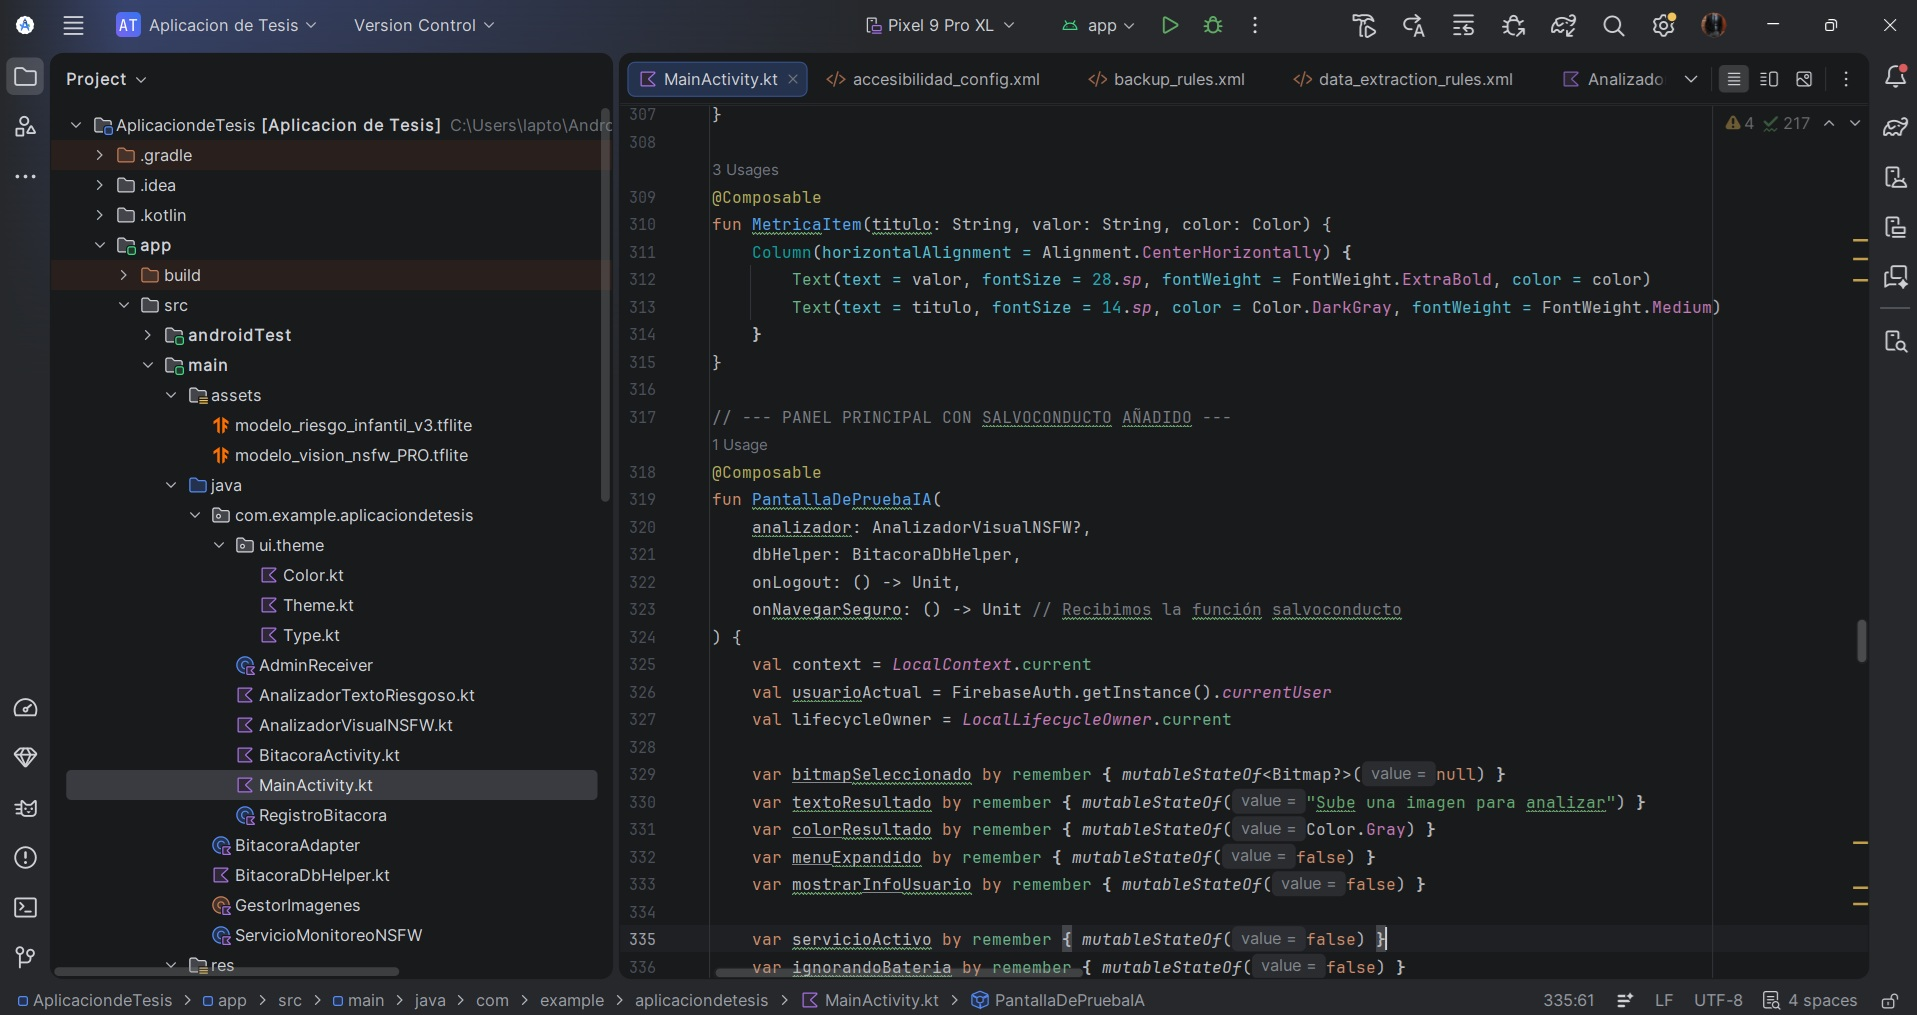
\includegraphics[width=0.8\textwidth]{Figures/Anexos/android_studio_tflite.jpg}
    \caption{Interfaz de Android Studio para la integración de modelos TensorFlow Lite en la aplicación móvil}
    \label{fig:anexo-android-studio}
\end{figure}

\begin{tcolorbox}[colback=gray!5!white, colframe=gray!60!black, title=Anexo B \- Documento de Validación por Especialista en \gls{ia} y Machine Learning]
    En este anexo se presenta el documento original que contiene el dictamen de validación técnica extendido por un especialista en Inteligencia Artificial y \textit{Machine Learning}. Este documento certifica formalmente el cumplimiento de las métricas algorítmicas, de rendimiento en hardware y de privacidad del sistema \textit{Parental AI Shield}.
\end{tcolorbox}

\begin{figure}[H]
    \centering
    % Asegúrate de subir tu PDF a la carpeta Figures/Anexos/ y poner el nombre correcto aquí
    \includegraphics[width=0.95\textwidth]{Figures/Anexos/validacion_tecnica.pdf}
    \caption{Documento de Validación Técnica firmado por el especialista}
    \label{fig:anexo-validacion}
\end{figure}

\clearpage


\clearpage

\begin{tcolorbox}[colback=gray!5!white, colframe=gray!60!black, title=Anexo C \- Código en Python para el diseño de la red neuronal \gls{nlp}]
    En este anexo se presenta un fragmento del código en Python utilizado para la arquitectura y entrenamiento del modelo de Procesamiento de Lenguaje Natural (Red Convolucional 1D) mediante la librería TensorFlow/Keras.
\end{tcolorbox}

\begin{listing}[H]
    \caption{Fragmento de código en Python para la generación y compilación del modelo \gls{nlp} Conv1D}
    \label{cod:anexo-modelo-nlp}
    \begin{minted}{python}
        import tensorflow as tf
        from tensorflow.keras.models import Sequential
        from tensorflow.keras.layers import Embedding, Conv1D, GlobalMaxPooling1D, Dense, Dropout

        # Definición de la arquitectura del modelo semántico
        modelo_nlp = Sequential([
            Embedding(input_dim=2000, output_dim=32, input_length=50),
            Dropout(0.4),
            Conv1D(filters=32, kernel_size=3, activation='relu'),
            GlobalMaxPooling1D(),
            Dense(16, activation='relu'),
            Dropout(0.4),
            Dense(1, activation='sigmoid') # Clasificación binaria (Seguro vs Riesgo)
        ])

        # Compilación del modelo
        modelo_nlp.compile(optimizer='adam', 
                           loss='binary_crossentropy', 
                           metrics=['accuracy'])
        
        modelo_nlp.summary()
    \end{minted}
\end{listing}

\clearpage

\begin{tcolorbox}[colback=gray!5!white, colframe=gray!60!black, title=Anexo D \- Fragmento de código en Python para el análisis de datos de validación]
    En este anexo se presenta un ejemplo del script estructurado utilizado para el análisis de los datos generados durante la prueba de campo (encuestas a padres) y la exportación vectorial de los gráficos estadísticos mostrados en el capítulo de Resultados. El código completo se encuentra disponible en los cuadernos de investigación adjuntos.
\end{tcolorbox}

\begin{listing}[H]
    \caption{Fragmento de código para el análisis de la matriz de respuestas y generación de gráficas con Seaborn}
    \label{cod:anexo-graficas-analisis}
    \begin{minted}{python}
        import pandas as pd
        import matplotlib.pyplot as plt
        import seaborn as sns

        # Leer archivo de resultados de la encuesta de validación
        df = pd.read_csv("Resultados_Evaluacion_Parental_AI.csv")

        # Extraer específicamente la columna de incidencias de Falsos Positivos
        falsos_positivos_df = df.iloc[:, 10].value_counts().reset_index()
        falsos_positivos_df.columns = ['Respuesta', 'Cantidad']

        # Asignación de la paleta de colores institucional
        PALETA = ["#2c3e50", "#3498db", "#e67e22"]
        colores_fp = [PALETA[0] if "Nunca" in str(r) else PALETA[2] 
                      for r in falsos_positivos_df['Respuesta']]

        # Generación de la visualización gráfica exportable a PDF (Vector)
        plt.figure(figsize=(8, 6))
        plt.pie(falsos_positivos_df['Cantidad'], 
                labels=falsos_positivos_df['Respuesta'], 
                autopct='%1.1f%%', 
                colors=colores_fp, 
                wedgeprops={'edgecolor': 'white', 'linewidth': 2})
                
        plt.title('Incidencia de Falsos Positivos durante la Prueba', pad=20)
        plt.savefig('grafica_falsos_positivos.pdf', format='pdf', bbox_inches='tight')
    \end{minted}
\end{listing}

\subsection{Entorno de Hardware y Estación de Trabajo}
Para el diseño de la arquitectura, el preprocesamiento de los \textit{datasets}, el entrenamiento de los modelos de Inteligencia Artificial (Procesamiento de Lenguaje Natural y Visión Artificial) y la compilación del código nativo, se empleó una estación de trabajo con capacidades de procesamiento acelerado. Las especificaciones técnicas del equipo principal se detallan a continuación:

\begin{itemize}
    \item \textbf{Procesador (\gls{cpu}):} [Intel Core i7-13620h]. Este componente fue fundamental para la compilación eficiente del proyecto mediante Gradle y la ejecución fluida de emuladores virtuales de Android durante la fase de depuración.
    \item \textbf{Memoria \gls{ram}:} [16 GB ] [DDR5]. Capacidad estrictamente necesaria para mantener en ejecución simultánea el Entorno de Desarrollo Integrado (Android Studio), los perfiladores de memoria (\textit{Android Profiler}) y los cuadernos de Python.
    \item \textbf{Procesamiento Gráfico (GPU):} [Ej. NVIDIA GeForce RTX 4070 de 8GB]. El uso de aceleración por hardware fue indispensable para reducir los tiempos de entrenamiento tensorial durante la fase de \textit{Fine-Tuning} de MobileNetV2 y la red Conv1D.
    \item \textbf{Almacenamiento:} Unidad de Estado Sólido (\gls{ssd}) de [1 TB], requerida para garantizar tiempos de lectura y escritura óptimos al manejar y cargar en memoria miles de imágenes y fragmentos de texto del conjunto de datos.
    \item \textbf{Sistema Operativo:} [ Windows 11].
\end{itemize}

Adicionalmente se utilizó un dispositivo movil simulado siendo este un emulador de Android (Pixel 9 Pro XL) con Android 14, configurado para replicar las condiciones de hardware de un smartphone de gama media-alta, con el fin de validar la eficiencia y el rendimiento del sistema \textit{Parental AI Shield} en un entorno realista.

\subsection{Enlace a Github del proyecto Latex}
https://github.com/Croximity/Tesis
